\documentclass[12pt]{article}

\usepackage{amsmath}
\usepackage{amsfonts}
\usepackage[margin=1in]{geometry}
\usepackage{graphicx}
\usepackage{epstopdf}
\graphicspath{ {quadratic_example/} }

\begin{document}

\section{Multiscale SDEs}

Consider the SDEs
\begin{eqnarray}
dx &=& adt + dW_1\\
dy &=& -\frac{y}{\epsilon} dt + \frac{1}{\sqrt{\epsilon}} dW_2
\end{eqnarray}

So $y$ is a fast noise whose equilibrium measure is bounded and $\mathcal{O}(1)$

Let $y = \frac{z}{\sqrt{\epsilon}}$. Then
\begin{eqnarray}
dx &=& adt + dW_1\\
dz &=& -\frac{z}{\epsilon} dt +  dW_2
\end{eqnarray}

Therefore, now $z$ is a stochastic variable whose diffusion is unity, and whose equilibrium measure is $\mathcal{O}(\epsilon)$. 
%
Therefore, when $\epsilon \ll 1$, we have that $z \ll x$, and so we will recover $x$ only.

This falls into a more general form of SDE
\begin{equation}
dx_i = a(X) dt + dW_i
\end{equation}
and we will let $X = \begin{bmatrix} X^1 \\ X^2 \\ \vdots \\ X^n \end{bmatrix}$

\section{Covariance Estimation}

Given $X$ governed by the above SDE, we can sample ``bursts'' around a point $X_0$ in order to estimate the covariance. 

These clouds will be distributed 

\begin{equation}
X \sim \mathcal{N}\left( X_0, \delta t I \right)
\end{equation}

Then
$$\int_{-\infty}^{\infty} d\mu(X) = \begin{bmatrix} 1 \\ \vdots \\ 1\end{bmatrix}$$
$$\int_{-\infty}^{\infty} X d\mu(X) = X_0$$
$$\int_{-\infty}^{\infty} X X^T d\mu(X) - \left( \int_{-\infty}^{\infty} X d\mu(X) \right) \left( \int_{-\infty}^{\infty} X d\mu(X) \right)^T = \delta t I$$


We now consider a function $\mathbf{f}: \mathbb{R}^n \mapsto \mathbb{R}^m$.
%
Let $f^i(X)$ denote the $i^{th}$ entry of $\mathbf{f}$, and let $f^i_j(X) = \frac{\partial f^i}{\partial X^j}$.
%
By Taylor expansion around $X=X_0$,
\begin{eqnarray}
f^i(X) &=& 
f^i(X_0) 
+ \sum_k f^i_k(X_0)  (X^k-X^k_0) 
+\frac{1}{2} \sum_{k,l}  f^i_{kl} (X_0) (X^k-X_0^k) (X^l-X_0^l) \\
&& + \frac{1}{6} \sum_{k,l,m} f^i_{klm} (X_0) (X^k-X_0^k) (X^l-X_0^l) (X^m-X_0^m) \\
&& + \frac{1}{24} \sum_{k,l,m,n} f^i_{klmn} (X_0) (X^k-X_0^k) (X^l-X_0^l) (X^m-X_0^m) (X^n-X_0^n) \\
&&+ \mathcal{O}\left( \| X- X_0 \|^5 \right)
\end{eqnarray}



We then estimate the covariance as
\begin{eqnarray}
\hat{C}^{ij} &=& 
\int_{-\infty}^{\infty} f^i(X) f^j(X) d\mu(X) - \left(\int_{-\infty}^{\infty} f^i(X) d\mu(X) \right) \left(\int_{-\infty}^{\infty} f^j(X) d\mu(X) \right) \\
&=&
\delta t \sum_k f^i_k(X_0)  f^j_k(X_0) 
+ \frac{\delta t^2}{2} \sum_k f^i_k(X_0) f^j_{kkk} (X_0)  
 + \frac{\delta t^2}{2} \sum_k f^i_{kkk} (X_0) f^j_k(X_0) \\
&&+  \frac{3 \delta t^2}{4} \sum_{k} f^i_{kk}(X_0) f^j_{kk}(X_0) 
- \frac{\delta t^2}{4} \left( \sum_k f^i_{kk}(X_0) \right) \left( \sum_k f^j_{kk}(X_0) \right) 
 + \mathcal{O}\left( \delta t^3 \right) \\
\end{eqnarray}

Let 
\begin{equation}
J_1(X_0) = \begin{bmatrix}
f_1^1 & f_2^1 & \dots & f_n^1 \\
\vdots & \vdots & \cdots & \vdots \\
f_1^m & f_2^m & \dots & f_n^m
\end{bmatrix}
\end{equation}

\begin{equation}
J_2(X_0) = \begin{bmatrix}
f_{11}^1 & f_{22}^1 & \dots & f_{nn}^1 \\
\vdots & \vdots & \cdots & \vdots \\
f_{11}^m & f_{22}^m & \dots & f_{nn}^m
\end{bmatrix}
\end{equation}

\begin{equation}
J_3(X_0) = \begin{bmatrix}
f_{111}^1 & f_{222}^1 & \dots & f_{nnn}^1 \\
\vdots & \vdots & \cdots & \vdots \\
f_{111}^m & f_{222}^m & \dots & f_{nnn}^m
\end{bmatrix}
\end{equation}

Then
\begin{eqnarray}
\hat{C}(X_0) &=& \delta t J_1 J_1^T 
+ \frac{\delta t^2}{2} \left[ J_1 J_3^T + J_3 J_1^T  
+ \frac{3}{2} J_2 J_2^T 
-\frac{1 }{2} J_2 1 1^T J_2^T \right]
+ \mathcal{O} (\delta t^3) %\\
%&=& \delta t J_1 J_1^T 
%+ \frac{\delta t^2}{2} U \Sigma V
%+ \mathcal{O} (\delta t^3)
\end{eqnarray}
%
In this equation, we see what we expect (a linear function of the variance, due to the gradient of $f$) and a second (higher-order) term arising from the curvature and third derivative of $f$.
%
The importance of this second term increases as the curvature increases, as well as when $\delta t$ increases. 



Then
\begin{equation}
\hat{C}^{-1}(X_0) \approx \frac{1}{\delta t} \left( J J^T \right)^{-1} - A
\end{equation}
%
where 
\begin{equation}
A = \frac{1}{2} (J_1 J_1^T)^{-1} U \left(\Sigma^{-1} + \frac{\delta t}{2} V \left( J_1 J_1^T \right)^{-1} U \right)^{-1} V \left( J_1 J_1^T \right)^{-1}
\end{equation}
and
\begin{equation}
U \Sigma V = J_1 J_3^T + J_3 J_1^T + \frac{3}{2} J_2 J_2^T -\frac{1 }{2} J_2 1 1^T J_2^T 
\end{equation}
$A$ is a function of the first-, second-, and third-order derivatives of $\mathbf{f}$.

\section{Mahalanobis Distance}


We now approximate the distances $\| X_2 - X_1 \|$.
%
Let $g = f^{-1}: \mathbb{R}^m \mapsto \mathbb{R}^n$, and let $Y_1 = f(X_1)$, and $Y_2 = f(X_2)$.
%
Again, we let $g_j^i = \frac{\partial g^i}{\partial Y^j}$.
%
Then, Taylor expansion around $Y_1$ gives
%
\begin{eqnarray}
X_2^i &=& X_1^i + \sum_j g_j^i (Y_1) (Y^j_2 - Y^j_1 ) 
+ \frac{1}{2} \sum_{kl}  g^i_{kl} (Y_1) (Y^k_2 - Y^k_1)(Y^l_2 - Y^l_1) \\
&&+ \frac{1}{6} \sum_{klm}  g^i_{klm} (Y_1) (Y^k_2 - Y^k_1)(Y^l_2 - Y^l_1) (Y^m_2 - Y^m_1) 
+ \mathcal{O}( \|Y_2 - Y_1\|^4 )
\end{eqnarray}
%
We can obtain a similar expression for expansion around $Y_2$.
%
We then compute $\| X_2 - X_1\|$ using both expansions, and average, to obtain
%
\begin{eqnarray}
&&\| X_2 - X_1 \|^2 \\
&=& \frac{1}{2} (Y_2 - Y_1 )^T ((J J^T)^{-1} (Y_1) + (J J^T)^{-1}(Y_2)) (Y_2 - Y_1 ) \\
&& + \frac{1}{2} \sum_{ijkl} \left( g_j^i (Y_1) g^i_{kl} (Y_1) - g_j^i (Y_2) g^i_{kl} (Y_2) \right) (Y^j_2 - Y^j_1 )  (Y^k_2 - Y^k_1)(Y^l_2 - Y^l_1) \\
&& + \frac{1}{8} \sum_{ijklm}  \left( g^i_{jk} (Y_1) g^i_{lm} (Y_1) + g^i_{jk} (Y_2) g^i_{lm} (Y_2)  \right) (Y^j_2 - Y^j_1) (Y^k_2 - Y^k_1) (Y^l_2 - Y^l_1) (Y^m_2 - Y^m_1) \\
&& + \frac{1}{6} \sum_{ijklm}  \left( g^i_{j} (Y_1) g^i_{klm} (Y_1) + g^i_{j} (Y_2) g^i_{klm} (Y_2)  \right)(Y^j_2 - Y^j_1) (Y^k_2 - Y^k_1) (Y^l_2 - Y^l_1) (Y^m_2 - Y^m_1) \\
&& + \mathcal{O} (\|Y_1 - Y_2 \|^6 ) 
\end{eqnarray}

Let 
$$K_1 = \sup_{i,j,Y} |g_j^i(Y)|$$
$$K_2 = \sup_{i,j,k,Y} |g_{jk}^i(Y)|$$
$$K_3 = \sup_{i,j,k,l,Y} |g_{jkl}^i(Y)|$$

Then, the error from Taylor expansion 
\begin{eqnarray}
&&\| X_2 - X_1 \|^2 \\
&\le&  \left| \frac{1}{2} (Y_2 - Y_1 )^T ((J J^T)^{-1} (Y_1) + (J J^T)^{-1}(Y_2)) (Y_2 - Y_1 ) \right| \\
&& + n \left( \left| K_1 K_2 \right| + \left| \frac{ K_2^2}{4} \right|  + \left| \frac{K_1 K_3}{3} \right|  \right) \| Y_2 - Y_1 \| ^4  \\
&& + \mathcal{O} (\|Y_1 - Y_2 \|^6 ) 
\end{eqnarray}

Our {\em estimate} of the distance is 
\begin{eqnarray}
&&\| X_2 - X_1 \|^2 \\
&=& \frac{\delta t}{2} (Y_2 - Y_1)^T (\hat{C}^{-1} (Y_1) + \hat{C}^{-1}(Y_2)) (Y_2 - Y_1)\\
&\approx & \frac{1}{2} (Y_2 - Y_1)^T \left((J J^T)^{-1}(Y_1)  + (J J^T)^{-1}(Y_2) \right) (Y_2 - Y_1) \\
&& - \frac{\delta t}{2} (Y_2 - Y_1)^T \left( A(Y_1) + A(Y_2) \right) (Y_2 - Y_1)
\end{eqnarray}

We therefore have two errors
\begin{itemize}
\item The error from the {\em estimation} of the covariance.
%
This is
$$\mathcal{O} \left( \delta t \| Y_2 - Y_1 \|^2 \sup_{Y, i} |\lambda_i(A(Y))| \right)$$
%
where $A$ is a function of the derivatives of $\mathbf{f}$, and $\lambda_i(A(Y))$ are the eigenvalues of $A(Y))$.

\item The errors from the truncation of the Taylor expansion for the Mahalanobis distance, which is 
$$\mathcal{O} \left(  n \left( \left| K_1 K_2 \right| + \left| \frac{ K_2^2}{4} \right|  + \left| \frac{K_1 K_3}{3} \right|  \right) \| Y_2 - Y_1 \| ^4  \right)$$
\end{itemize}

We want to set the scale of the kernel such that both of these errors are smaller than
\begin{equation}
(Y_2 - Y_1)^T (JJ^T)^{-1} (Y_2 - Y_1) 
\end{equation}

\section{Example}

\subsection{Equations}

Define the following two-dimensional system of SDEs
\begin{eqnarray}
dX(1) &=& 3 dt + dW_1 \\ 
dX(2) &=& \frac{-X(2)}{\epsilon} dt + dW_2 
\end{eqnarray}
where $W_1, W_2$ are independent Brownian motions, and $\epsilon \ll 1$.

Let
\begin{eqnarray}
f^1(X) &=& X(1) + \frac{ X(2)^2}{\epsilon} \\
f^2(X) &=& \frac{X(2)}{\sqrt{\epsilon}}
\end{eqnarray}
Therefore, $X(2)$ is now a ``fast'' variable, and we have further applied a nonlinear transformation to this fast-slow system. 

The inverse function $g = f^{-1}$ is
\begin{eqnarray}
g^1(Y) &=& Y(1) - Y(2)^2 \\
g^2(Y) &=& Y(2) \sqrt{\epsilon}
\end{eqnarray}

The three relevant quantities for NIVs are 
\begin{itemize}
\item The linearized approximation to the distance,
%
\begin{equation}
(Y_2 - Y_1)^T (JJ^T)^{-1} (Y_2 - Y_1) 
\approx \mathcal{O} \left(  \frac{1}{2} \left( 2 + \epsilon + \sqrt{ 9 + 2 \epsilon + \epsilon^2}\right) \Delta Y^2\right) 
\end{equation}
where $\Delta Y =  \|Y_2 - Y_1\|$

\item The error from the {\em estimation} of the covariance.
%
This is
\begin{equation}
\mathcal{O} \left( \delta t \| Y_2 - Y_1 \|^2 \sup_{Y, i} |\lambda_i(A(Y))| \right) 
= \mathcal{O} \left( \frac{38 \delta t}{\epsilon ^2 + 2 \delta t}\Delta Y^2 \right)
\end{equation}

\item The errors from the {\em truncation} of the Taylor expansion for the Mahalanobis distance, which is 
\begin{equation}
\mathcal{O} \left(  n \left( \left| K_1 K_2 \right| + \left| \frac{ K_2^2}{4} \right|  + \left| \frac{K_1 K_3}{3} \right|  \right) \| Y_2 - Y_1 \| ^4  \right)
= \mathcal{O} \left( 10 \Delta Y^4  \right) 
\end{equation}

\end{itemize}

We want the two error terms to be small relative to the distance approximation. 
%
We therefore choose the scale of the diffusion maps kernel $\sigma_{kernel}$ such that
\begin{equation}
\sigma_{kernel} = \mathcal{O} \left(  \frac{1}{2} \left( 2 + \epsilon + \sqrt{ 9 + 2 \epsilon + \epsilon^2}\right) \Delta Y^2\right)
\end{equation}
%
corresponding to a $\Delta Y$ where
\begin{equation}
  \frac{1}{2} \left( 2 + \epsilon + \sqrt{ 9 + 2 \epsilon + \epsilon^2}\right) \Delta Y^2  
\gg 
\max \left\{  
\frac{38 \delta t}{\epsilon ^2 + 2 \delta t} \Delta Y^2, 
10 \Delta Y^4
 \right\}
\end{equation}

\subsection{Results}

We did five different simulations to look at the effects of $\epsilon$, $\sigma_{kernel}$, and $\delta t$ on the results.
%
We can see that we recover the correct variable (consistent with DMAPS) if the errors in the covariance estimation and the Taylor expansion are smaller than the linear approximation to the distance. 

\begin{table}
\begin{tabular}{r | c c c}
Simulation number & $\epsilon$ & $\sigma_{kernel}$ & $\delta t$ \\
\hline
1 & $10^{-3}$ & $10^{-2}$ & $10^{-8}$ \\
2 & $10^{-3}$ & $10^{2}$ & $10^{-8}$ \\
3 & $10^{-3}$ & $10^{-2}$ & $10^{-5}$ \\
4 & $10^{-4}$ & $10^{-2}$ & $10^{-10}$ \\
5 & $10^{-4}$ & $10^{-2}$ & $10^{-5}$ 
\end{tabular}
\caption{Parameter values for different simulation experiments. }
\end{table}


\begin{figure}
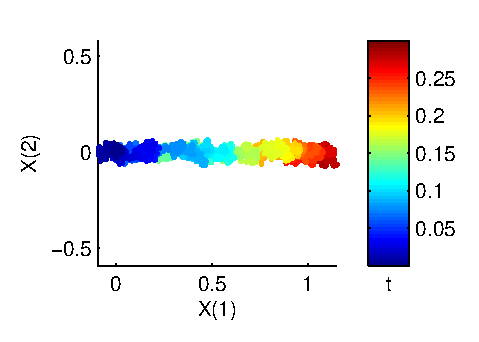
\includegraphics[width=0.22\textwidth]{orig_data_1}
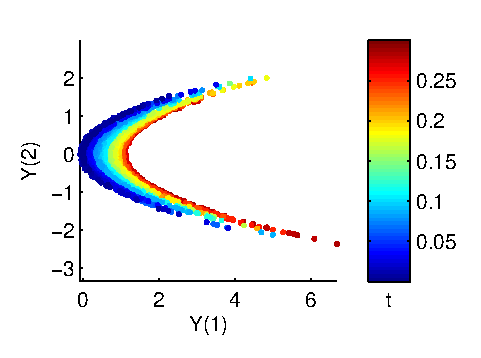
\includegraphics[width=0.22\textwidth]{function_data_1}
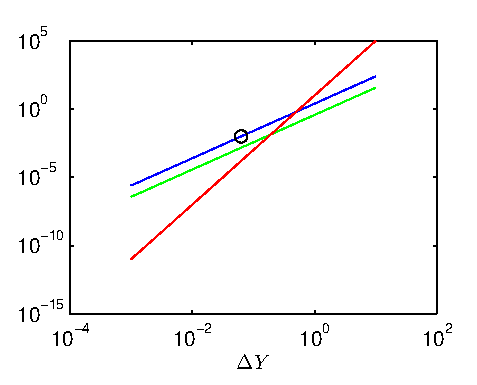
\includegraphics[width=0.22\textwidth]{error_terms_1}
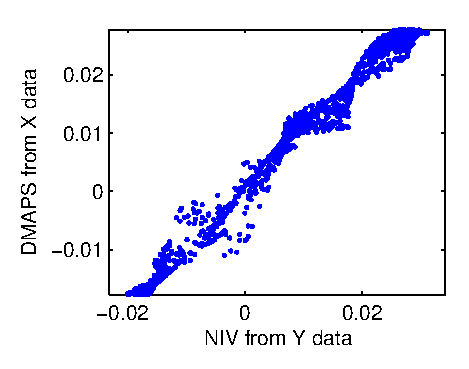
\includegraphics[width=0.22\textwidth]{dmaps_corr_1} \\
%
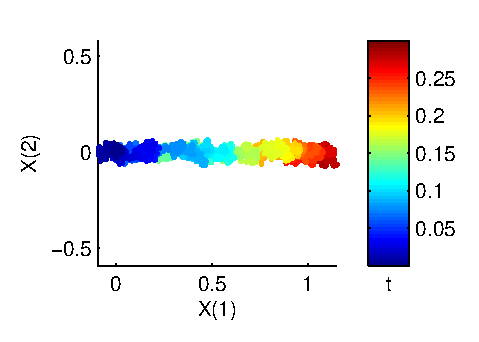
\includegraphics[width=0.22\textwidth]{orig_data_2}
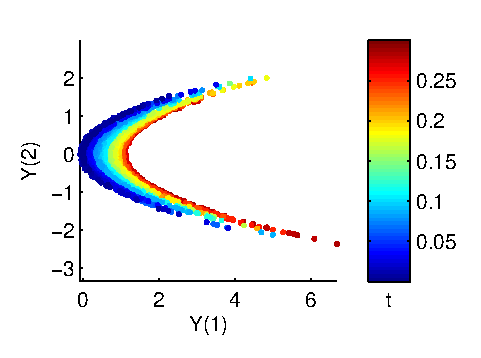
\includegraphics[width=0.22\textwidth]{function_data_2}
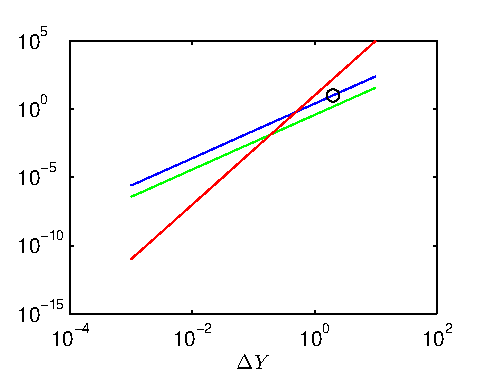
\includegraphics[width=0.22\textwidth]{error_terms_2}
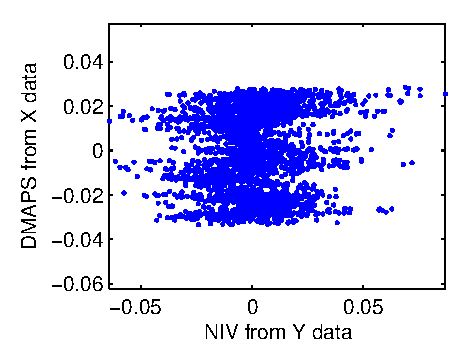
\includegraphics[width=0.22\textwidth]{dmaps_corr_2} \\
%
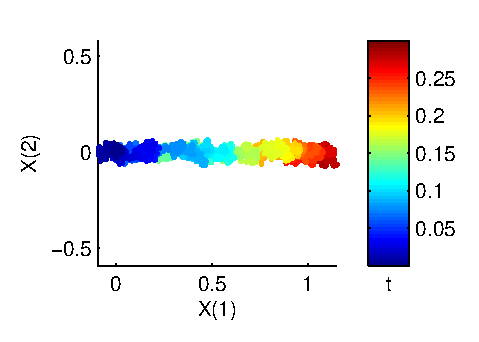
\includegraphics[width=0.22\textwidth]{orig_data_3}
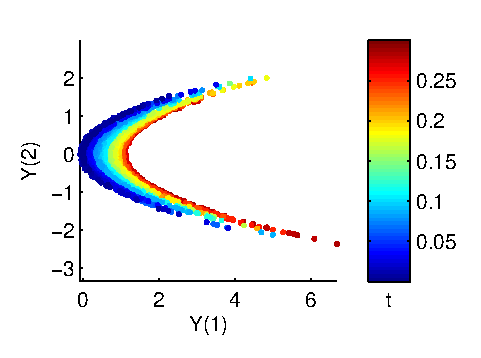
\includegraphics[width=0.22\textwidth]{function_data_3}
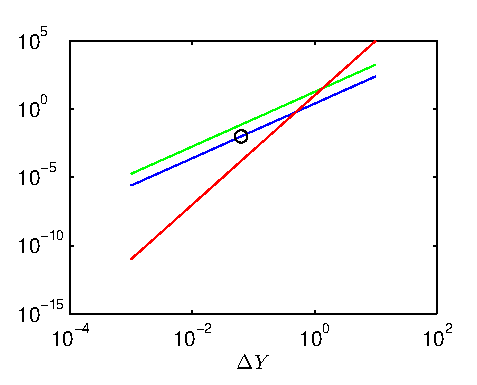
\includegraphics[width=0.22\textwidth]{error_terms_3}
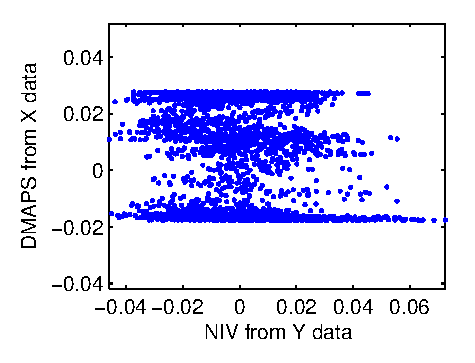
\includegraphics[width=0.22\textwidth]{dmaps_corr_3} \\
%
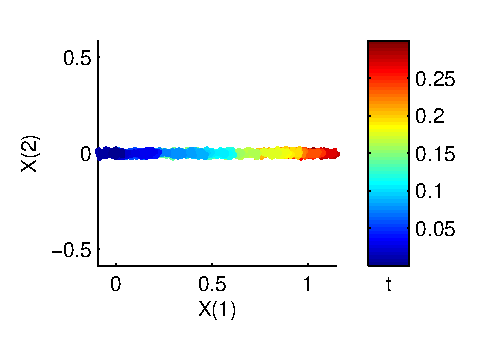
\includegraphics[width=0.22\textwidth]{orig_data_4}
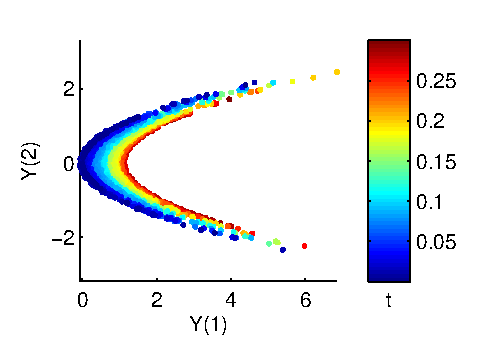
\includegraphics[width=0.22\textwidth]{function_data_4}
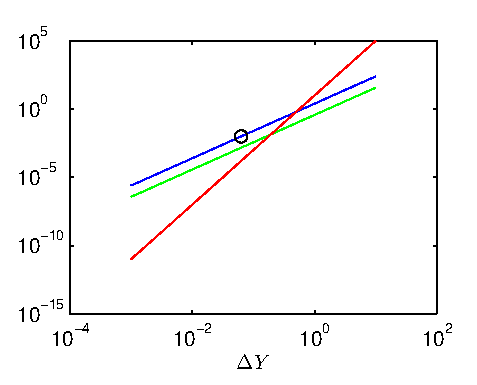
\includegraphics[width=0.22\textwidth]{error_terms_4}
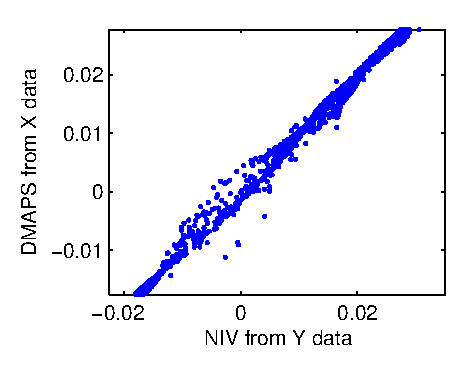
\includegraphics[width=0.22\textwidth]{dmaps_corr_4} \\
%
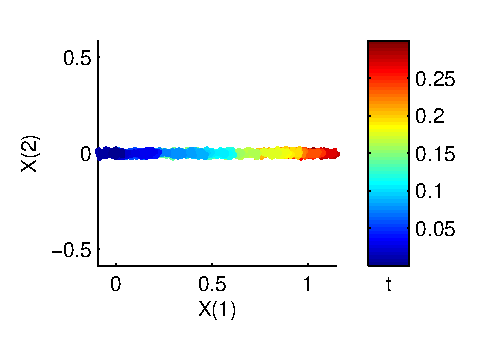
\includegraphics[width=0.22\textwidth]{orig_data_5}
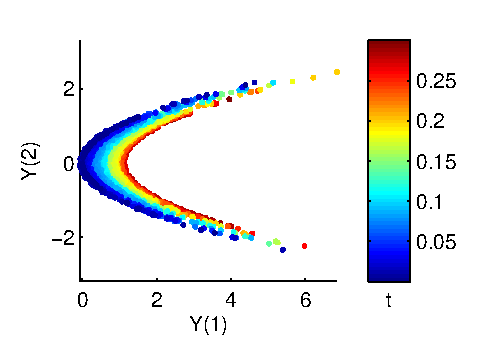
\includegraphics[width=0.22\textwidth]{function_data_5}
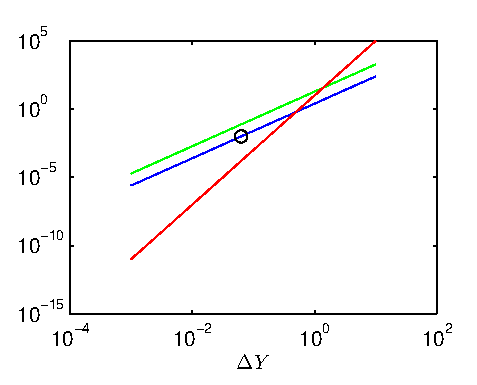
\includegraphics[width=0.22\textwidth]{error_terms_5}
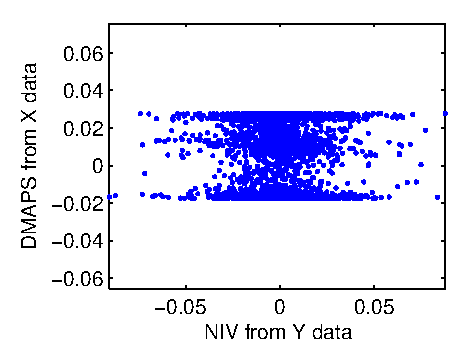
\includegraphics[width=0.22\textwidth]{dmaps_corr_5}
\caption{(First column) Original data $X$. (Second column) Transformed data $Y = f(X)$. (Third column) Relevant quantities as a function of $\Delta Y$. The blue curve is the linear approximation distance, the green curve is the error from covariance estimation, and the red curve is the error from Taylor expansion. The blue circle indicates the value of $\sigma_{kernel}$ used in the diffusion maps calculations. (Fourth column) The first NIV, obtained from the transformed data $Y$, versus the first DMAPS variable, obtained from the original data $X$. }
\end{figure}

\subsection{Empirical Estimation}

Again, we have the three terms in our expansion
\begin{itemize}
\item The linearized approximation to the distance,
%
\begin{equation}
(Y_2 - Y_1)^T (JJ^T)^{-1} (Y_2 - Y_1) 
\end{equation}

\item The error from the {\em estimation} of the covariance.
%
This is
\begin{equation}
\mathcal{O} \left( \delta t \| Y_2 - Y_1 \|^2 \sup_{Y, i} |\lambda_i(A(Y))| \right) 
\end{equation}

\item The errors from the {\em truncation} of the Taylor expansion for the Mahalanobis distance, which is 
\begin{equation}
\mathcal{O} \left(  n \left( \left| K_1 K_2 \right| + \left| \frac{ K_2^2}{4} \right|  + \left| \frac{K_1 K_3}{3} \right|  \right) \| Y_2 - Y_1 \| ^4  \right) 
\end{equation}

\end{itemize}
and we want to choose $\sigma_{kernel}$ such that the first term dominates. 

When we calculate the distances, we measure a sum of the three terms
\begin{eqnarray}
\| X_2 - X_1 \|^2_{est} &=& 
(Y_2 - Y_1)^T (JJ^T)^{-1} (Y_2 - Y_1)  \\
&&
+ \mathcal{O} \left( \delta t \| Y_2 - Y_1 \|^2 \sup_{Y, i} |\lambda_i(A(Y))| \right) \\
&& + \mathcal{O} \left(  n \left( \left| K_1 K_2 \right| + \left| \frac{ K_2^2}{4} \right|  + \left| \frac{K_1 K_3}{3} \right|  \right) \| Y_2 - Y_1 \| ^4  \right) 
\end{eqnarray}

Therefore, when the first term dominates, we expect
\begin{itemize}
\item $\| X_2 - X_1 \|^2_{est} \sim \| Y_2 - Y_1 \|^2$ (so that the truncation error from the Taylor expansion is not too large)
\item $\| X_2 - X_1 \|^2_{est}$ constant as a function of $\delta t$ (so that the error from the covariance estimation is not too large)
\end{itemize}


We can look at this for this specific example, with $\epsilon = 10^{-3}$. 
%
We use a cloud of $200$ data points to estimate each covariance matrix. 


\begin{figure}

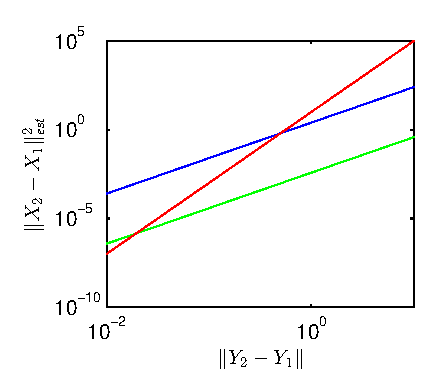
\includegraphics[width=0.3\textwidth]{errors_function_dy}
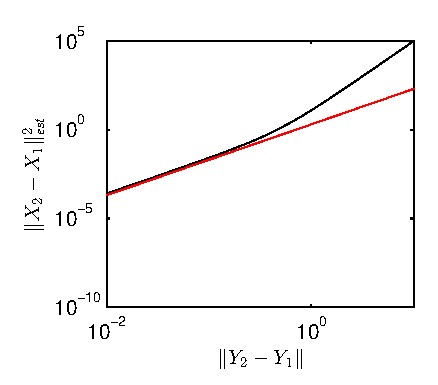
\includegraphics[width=0.3\textwidth]{totaldist_function_dy}
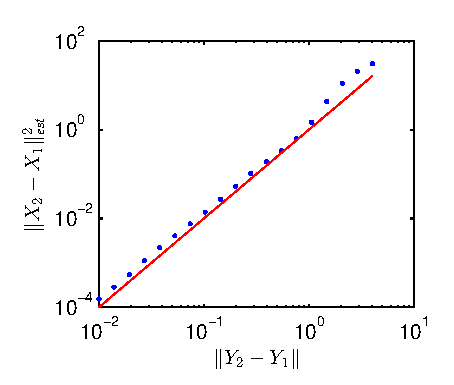
\includegraphics[width=0.3\textwidth]{empirical_totaldist_function_dy}

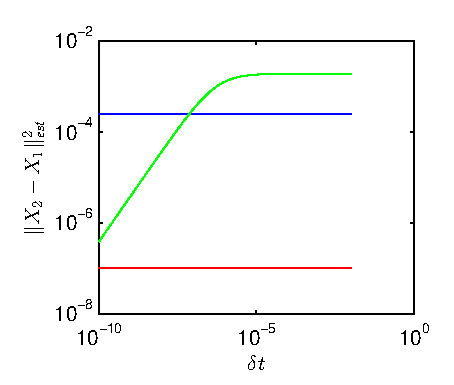
\includegraphics[width=0.3\textwidth]{errors_function_dt}
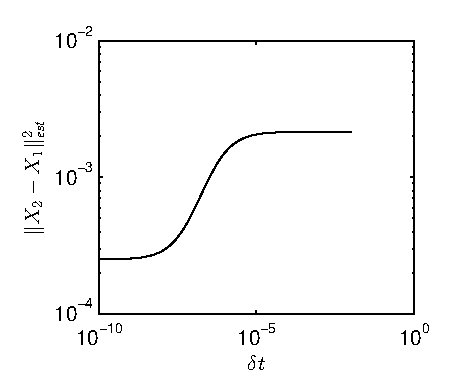
\includegraphics[width=0.3\textwidth]{totaldist_function_dt}
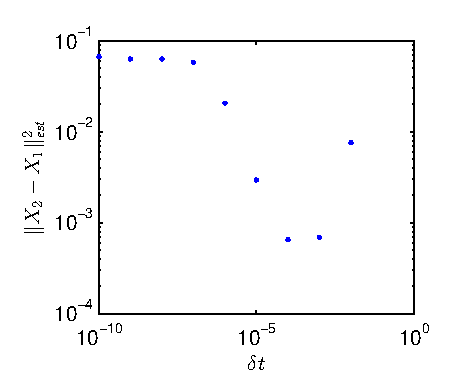
\includegraphics[width=0.3\textwidth]{empirical_totaldist_function_dt}

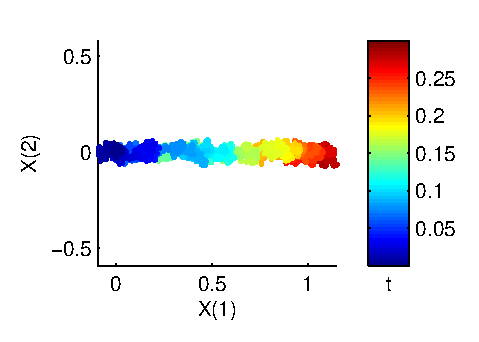
\includegraphics[width=0.3\textwidth]{original_data}
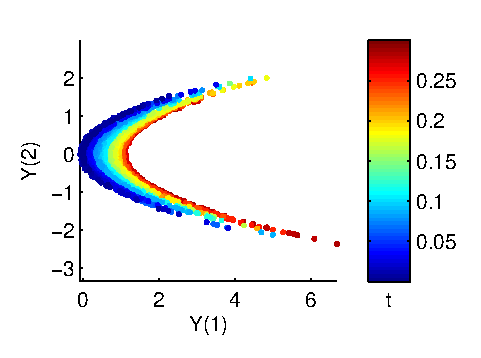
\includegraphics[width=0.3\textwidth]{transformed_data}
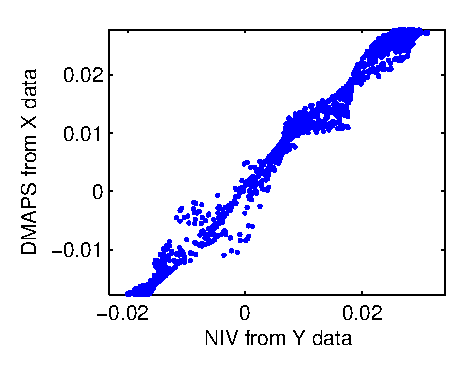
\includegraphics[width=0.3\textwidth]{NIV_correlation}

\caption{(Top row, left) Relevant quantities as a function of $\|Y_2 - Y_1\|$, with $\delta t = 10^{-10}$. The blue curve is the linear approximation distance, the green curve is the error from covariance estimation, and the red curve is the error from Taylor expansion.  (Center) The black curve denotes the sum of the three terms as a function of $\|Y_2 - Y_1\|$. The red curve is the $\|X_2 - X_1\|^2 = \|Y_2 - Y_1\|^2$ line. (Right) The blue points are the empirical $\| X_2 - X_1 \|$ as a function of $\|Y_2 - Y_1\|$. The red curve is the $\| X_2 - X_1 \|^2 = \|Y_2 - Y_1\|^2$ line. (Center row, left) Relevant quantities as a function of $\delta t$, with $\|Y_2 - Y_1\| = 0.01$. The blue curve is the linear approximation distance, the green curve is the error from covariance estimation, and the red curve is the error from Taylor expansion. (Center) The sum of the three terms as a function of $\delta t$. (Right) The empirical $\| X_2 - X_1 \|^2$ as a function of $\|Y_2 - Y_1\|$. (Bottom row, left) Original data $X$. (Center) Transformed data $Y = f(X)$. (Right) The first NIV, obtained from the transformed data $Y$, versus the first DMAPS variable, obtained from the original data $X$. Based on the results of how $\| X_2 - X_1 \|^2_{est}$ varies with $\| Y_2 - Y_1\|$ and $\delta t$, we choose $\sigma_{kernel} = 0.01$ and $\delta t = 10^{-9}$. }
\end{figure}



\appendix

\section{Algebra}

\subsection{Covariance estimation}

First order moment
\begin{eqnarray}
&&\int_{-\infty}^{\infty} f^i(X) d\mu(X) \\
&= & \int_{-\infty}^{\infty} \left[ f^i(X_0) + \sum_k f^i_k(X_0) (X^k-X_0^k)  + \frac{1}{2} \sum_{k,l} f^i_{kl}(X_0) (X^k-X_0^k) (X^l-X_0^l)  \right. \\
&& + \frac{1}{6} \sum_{k,l,m} f^i_{klm} (X_0) (X^k-X_0^k) (X^l-X_0^l) (X^m-X_0^m) \\
&& \left. + \frac{1}{24} \sum_{k,l,m,n} f^i_{klmn} (X_0) (X^k-X_0^k) (X^l-X_0^l) (X^m-X_0^m) (X^n-X_0^n)
+ \mathcal{O}\left( \| X- X_0 \|^5 \right) \right] d\mu(X) \\
&=& f^i(X_0) + \frac{1}{2} \sum_k f^i_{kk}(X_0) \delta t + \frac{\delta t^2}{8} \sum_{k} f^i_{kkkk} (X_0) + \mathcal{O} (\delta t^3 )
\end{eqnarray}

Second order moment
\begin{eqnarray}
&&\int_{-\infty}^{\infty} f^i(X) f^j(X) d\mu(X) \\
&= &
\int_{-\infty}^{\infty} \left[ f^i(X_0) + \sum_k f^i_k(X_0) (X^k-X_0^k)  + \frac{1}{2} \sum_{k,l} f^i_{kl}(X_0) (X^k-X_0^k) (X^l-X_0^l) \right. \\
&&  + \frac{1}{6} \sum_{k,l,m} f^i_{klm} (X_0) (X^k-X_0^k) (X^l-X_0^l) (X^m-X_0^m) \\
&& \left. + \frac{1}{24} \sum_{k,l,m,n} f^i_{klmn} (X_0) (X^k-X_0^k) (X^l-X_0^l) (X^m-X_0^m) (X^n-X_0^n)
+ \mathcal{O}\left( \| X- X_0 \|^5 \right) \right]  \\
&& \left[ f^j(X_0) + \sum_k f^j_k(X_0) (X^k-X_0^k)  + \frac{1}{2} \sum_{k,l} f^j_{kl}(X_0) (X^k-X_0^k) (X^l-X_0^l)  \right. \\
&&  + \frac{1}{6} \sum_{k,l,m} f^j_{klm} (X_0) (X^k-X_0^k) (X^l-X_0^l) (X^m-X_0^m)  \\
&&  \left. + \frac{1}{24} \sum_{k,l,m,n} f^j_{klmn} (X_0) (X^k-X_0^k) (X^l-X_0^l) (X^m-X_0^m) (X^n-X_0^n)
+ \mathcal{O}\left( \| X- X_0 \|^5 \right) \right]  d\mu(X) 
\end{eqnarray}

\begin{eqnarray}
&=& \int_{-\infty}^{\infty} \left[ 
f^i(X_0) f^j(X_0) \right. \\
&&+ f^i(X_0) \sum_k f^j_k(X_0) (X^k-X_0^k) 
+ f^j(X_0) \sum_k f^i_k(X_0) (X^k-X_0^k) \\
&& + \left(  \sum_k f^i_k(X_0) (X^k-X_0^k)  \right) \left(  \sum_k f^j_k(X_0) (X^k-X_0^k)  \right) \\
&& \left. + \frac{f^i(X_0)}{2} \sum_{k,l} f^j_{kl}(X_0) (X^k-X_0^k) (X^l-X_0^l) 
+ \frac{f^j(X_0)}{2} \sum_{k,l} f^i_{kl}(X_0) (X^k-X_0^k) (X^l-X_0^l)  \right. \\
&& + \frac{f^i(X_0)}{6} \sum_{k,l,m} f^j_{klm} (X_0) (X^k-X_0^k) (X^l-X_0^l) (X^m-X_0^m) \\
&& + \frac{f^j(X_0)}{6} \sum_{k,l,m} f^i_{klm} (X_0) (X^k-X_0^k) (X^l-X_0^l) (X^m-X_0^m) \\
&& + \left(\sum_k f^i_k(X_0) (X^k-X_0^k) \right) \left( \frac{f^j(X_0)}{2} \sum_{k,l} f^j_{kl}(X_0) (X^k-X_0^k) (X^l-X_0^l)  \right) \\
&& + \left(\sum_k f^j_k(X_0) (X^k-X_0^k) \right) \left( \frac{f^i(X_0)}{2} \sum_{k,l} f^j_{kl}(X_0) (X^k-X_0^k) (X^l-X_0^l)  \right)\\
&&+ \frac{f^i(X_0) }{24} \sum_{k,l,m,n} f^j_{klmn} (X_0) (X^k-X_0^k) (X^l-X_0^l) (X^m-X_0^m) (X^n-X_0^n) \\
&& + \frac{f^j(X_0) }{24} \sum_{k,l,m,n} f^i_{klmn} (X_0) (X^k-X_0^k) (X^l-X_0^l) (X^m-X_0^m) (X^n-X_0^n) \\
&& + \left( \sum_k f^i_k(X_0) (X^k-X_0^k) \right) \left( \frac{1}{6} \sum_{k,l,m} f^j_{klm} (X_0) (X^k-X_0^k) (X^l-X_0^l) (X^m-X_0^m)  \right) \\
&& + \left( \sum_k f^j_k(X_0) (X^k-X_0^k) \right) \left( \frac{1}{6} \sum_{k,l,m} f^i_{klm} (X_0) (X^k-X_0^k) (X^l-X_0^l) (X^m-X_0^m)  \right) \\
&&+ \left( \frac{1}{2} \sum_{k,l} f^i_{kl}(X_0) (X^k-X_0^k) (X^l-X_0^l)  \right) \left( \frac{1}{2} \sum_{k,l} f^j_{kl}(X_0) (X^k-X_0^k) (X^l-X_0^l)  \right) \\
&&\left. + \mathcal{O}\left( \| X- X_0 \|^5 \right) \right] d\mu(X) \\
 \end{eqnarray}
 
\begin{eqnarray}
&=& 
f^i(X_0) f^j(X_0)  + \delta t \sum_k f^i_k(X_0)  f^j_k(X_0) \\
&&  + \frac{f^i(X_0) \delta t}{2} \sum_{k} f^j_{kk}(X_0)
+ \frac{f^j(X_0) \delta t}{2} \sum_{k} f^i_{kk}(X_0)  \\
&&+ \frac{f^i(X_0) \delta t^2}{8} \sum_{k} f^j_{kkkk} (X_0) 
 + \frac{f^j(X_0) \delta t^2}{8} \sum_{k} f^i_{kkkk} (X_0)\\
&& + \frac{\delta t^2}{2} \sum_k f^i_k(X_0) f^j_{kkk} (X_0)  
 + \frac{\delta t^2}{2} \sum_k  f^i_{kkk} (X_0) f^j_k(X_0) \\
&&+  \frac{3  \delta t^2}{4} \sum_{k} f^i_{kk}(X_0) f^j_{kk}(X_0) 
 + \mathcal{O}\left( \delta t^3 \right) 
\end{eqnarray}

Covariance
\begin{eqnarray}
&& \hat{C}^{ij} = \\ 
&& \int_{-\infty}^{\infty} f^i(X) f^j(X) d\mu(X) - \left(\int_{-\infty}^{\infty} f^i(X) d\mu(X) \right) \left(\int_{-\infty}^{\infty} f^j(X) d\mu(X) \right) \\
&=& \left( f^i(X_0) f^j(X_0) 
 + \delta t \sum_k f^i_k(X_0)  f^j_k(X_0) \right.   \\
&&  + \frac{f^i(X_0) \delta t}{2} \sum_{k} f^j_{kk}(X_0)
+ \frac{f^j(X_0) \delta t}{2} \sum_{k} f^i_{kk}(X_0)  \\
&&+ \frac{f^i(X_0) \delta t^2}{8} \sum_{k} f^j_{kkkk} (X_0) 
+ \frac{f^j(X_0) \delta t^2}{8} \sum_{k} f^i_{kkkk} (X_0)\\
&& + \frac{\delta t^2}{2} \sum_k f^i_k(X_0) f^j_{kkk} (X_0)  
 + \frac{\delta t^2}{2} \sum_k f^i_{kkk} (X_0) f^j_k(X_0) \\
&&+  \frac{3  \delta t^2}{4} \sum_{k} f^i_{kk}(X_0) f^j_{kk}(X_0) 
 \left.+ \mathcal{O}\left( \delta t^3 \right) \right) \\
&&- \left( f^i(X_0) + \frac{1}{2} \sum_k f^i_{kk}(X_0) \delta t + \frac{\delta t^2}{8} \sum_{k} f^i_{kkkk} (X_0) + \mathcal{O} (\delta t^3 ) \right) \\
&&\left( f^j(X_0) + \frac{1}{2} \sum_k f^j_{kk}(X_0) \delta t + \frac{\delta t^2}{8} \sum_{k} f^j_{kkkk} (X_0) + \mathcal{O} (\delta t^3 ) \right) \\
&=&
\delta t \sum_k f^i_k(X_0)  f^j_k(X_0) 
+ \frac{\delta t^2}{2} \sum_k f^i_k(X_0) f^j_{kkk} (X_0)  
 + \frac{\delta t^2}{2} \sum_k f^i_{kkk} (X_0) f^j_k(X_0) \\
&&+  \frac{3 \delta t^2}{4} \sum_{k} f^i_{kk}(X_0) f^j_{kk}(X_0) 
- \frac{\delta t^2}{4} \left( \sum_k f^i_{kk}(X_0) \right) \left( \sum_k f^j_{kk}(X_0) \right) 
 + \mathcal{O}\left( \delta t^3 \right) 
\end{eqnarray}

Inverse covariance (by the Woodbury matrix identity)
\begin{eqnarray}
\hat{C}^{-1}(X_0) &\approx & 
\left( \delta t J_1 J_1^T + \frac{\delta t^2}{2}  U \Sigma V \right)^{-1} \\
&=& \left( \delta t J_1 J_1^T \right)^{-1} - 
\left( \delta t J_1 J_1^T \right)^{-1} \frac{\delta t^2}{2} U \left(\Sigma^{-1} + \frac{\delta t^2}{2} V \left( \delta t J_1 J_1^T \right)^{-1} U \right)^{-1} V \left( \delta t J_1 J_1^T \right)^{-1} \\
&=& \frac{1}{\delta t} \left( J J^T \right)^{-1}
- \frac{1}{2} (J_1 J_1^T)^{-1} U \left(\Sigma^{-1} + \frac{\delta t}{2} V \left( J_1 J_1^T \right)^{-1} U \right)^{-1} V \left( J_1 J_1^T \right)^{-1}  \\
&=& \frac{1}{\delta t} \left( J J^T \right)^{-1} - A
\end{eqnarray}
%
where 
\begin{equation}
A = \frac{1}{2} (J_1 J_1^T)^{-1} U \left(\Sigma^{-1} + \frac{\delta t}{2} V \left( J_1 J_1^T \right)^{-1} U \right)^{-1} V \left( J_1 J_1^T \right)^{-1}
\end{equation}
 and is a function of the first-, second-, and third-order derivatives of $\mathbf{f}$.

\subsection{Distance estimation}

\begin{eqnarray}
X_2^i &=& X_1^i + \sum_j g_j^i (Y_1) (Y^j_2 - Y^j_1 ) 
+ \frac{1}{2} \sum_{kl}  g^i_{kl} (Y_1) (Y^k_2 - Y^k_1)(Y^l_2 - Y^l_1) \\
&&+ \frac{1}{6} \sum_{klm}  g^i_{klm} (Y_1) (Y^k_2 - Y^k_1)(Y^l_2 - Y^l_1) (Y^m_2 - Y^m_1) 
+ \mathcal{O}( \|Y_2 - Y_1\|^4 )
\end{eqnarray}

Then computing the distance
\begin{eqnarray}
&&\| X_2 - X_1 \|^2 \\
&=&  \sum_i (X_2^i - X_1^i)^2 \\
&=& \sum_i  \left( \sum_j g_j^i (Y_1) (Y^j_2 - Y^j_1 )  \right.
+ \frac{1}{2} \sum_{kl}  g^i_{kl} (Y_1) (Y^k_2 - Y^k_1)(Y^l_2 - Y^l_1) \\
&&+ \left.  \frac{1}{6} \sum_{klm}  g^i_{klm} (Y_1) (Y^k_2 - Y^k_1)(Y^l_2 - Y^l_1) (Y^m_2 - Y^m_1) 
 + \mathcal{O}( \|Y_2 - Y_1\|^4 ) \right)^2 \\
&=& \sum_{ijk} g_j^i (Y_1) g_k^i (Y_1) (Y^j_2 - Y^j_1 ) (Y^k_2 - Y^k_1 ) \\
&& + \sum_{ijkl} g_j^i (Y_1) g^i_{kl} (Y_1) (Y^j_2 - Y^j_1 )  (Y^k_2 - Y^k_1)(Y^l_2 - Y^l_1) \\
&& + \frac{1}{4} \sum_{ijklm}  g^i_{jk} (Y_1) g^i_{lm} (Y_1) (Y^j_2 - Y^j_1) (Y^k_2 - Y^k_1) (Y^l_2 - Y^l_1) (Y^m_2 - Y^m_1) \\
&& + \frac{1}{3} \sum_{ijklm}  g^i_{j} (Y_1) g^i_{klm} (Y_1) (Y^j_2 - Y^j_1) (Y^k_2 - Y^k_1) (Y^l_2 - Y^l_1) (Y^m_2 - Y^m_1) \\
&& + \mathcal{O} (\|Y_1 - Y_2 \|^5 )
\end{eqnarray}

Expanding around $X_2$ yields
\begin{eqnarray}
&&\| X_2 - X_1 \|^2 \\
&=&  \sum_i (X_2^i - X_1^i)^2 \\
&=& \sum_{ijk} g_j^i (Y_2) g_k^i (Y_2) (Y^j_2 - Y^j_1 ) (Y^k_2 - Y^k_1 ) \\
&& - \sum_{ijkl} g_j^i (Y_2) g^i_{kl} (Y_2) (Y^j_2 - Y^j_1 )  (Y^k_2 - Y^k_1)(Y^l_2 - Y^l_1) \\
&& + \frac{1}{4} \sum_{ijklm}  g^i_{jk} (Y_2) g^i_{lm} (Y_2) (Y^j_2 - Y^j_1) (Y^k_2 - Y^k_1) (Y^l_2 - Y^l_1) (Y^m_2 - Y^m_1) \\
&& + \frac{1}{3} \sum_{ijklm}  g^i_{j} (Y_2) g^i_{klm} (Y_2) (Y^j_2 - Y^j_1) (Y^k_2 - Y^k_1) (Y^l_2 - Y^l_1) (Y^m_2 - Y^m_1) \\
&& + \mathcal{O} (\|Y_1 - Y_2 \|^5 )
\end{eqnarray}

Averaging the two expansions yields
\begin{eqnarray}
&&\| X_2 - X_1 \|^2 \\
&=&  \sum_i (X_2^i - X_1^i)^2 \\
&=& \frac{1}{2} \sum_{ijk} \left( g_j^i (Y_1) g_k^i (Y_1) + g_j^i (Y_2) g_k^i (Y_2) \right) (Y^j_2 - Y^j_1 ) (Y^k_2 - Y^k_1 ) \\
&& + \frac{1}{2} \sum_{ijkl} \left( g_j^i (Y_1) g^i_{kl} (Y_1) - g_j^i (Y_2) g^i_{kl} (Y_2) \right) (Y^j_2 - Y^j_1 )  (Y^k_2 - Y^k_1)(Y^l_2 - Y^l_1) \\
&& + \frac{1}{8} \sum_{ijklm}  \left( g^i_{jk} (Y_1) g^i_{lm} (Y_1) + g^i_{jk} (Y_2) g^i_{lm} (Y_2)  \right) (Y^j_2 - Y^j_1) (Y^k_2 - Y^k_1) (Y^l_2 - Y^l_1) (Y^m_2 - Y^m_1) \\
&& + \frac{1}{6} \sum_{ijklm}  \left( g^i_{j} (Y_1) g^i_{klm} (Y_1) + g^i_{j} (Y_2) g^i_{klm} (Y_2)  \right)(Y^j_2 - Y^j_1) (Y^k_2 - Y^k_1) (Y^l_2 - Y^l_1) (Y^m_2 - Y^m_1) \\
&& + \mathcal{O} (\|Y_1 - Y_2 \|^6 ) \\
&=& \frac{1}{2} (Y_2 - Y_1 )^T ((J J^T)^{-1} (Y_1) + (J J^T)^{-1}(Y_2)) (Y_2 - Y_1 ) \\
&& + \frac{1}{2} \sum_{ijkl} \left( g_j^i (Y_1) g^i_{kl} (Y_1) - g_j^i (Y_2) g^i_{kl} (Y_2) \right) (Y^j_2 - Y^j_1 )  (Y^k_2 - Y^k_1)(Y^l_2 - Y^l_1) \\
&& + \frac{1}{8} \sum_{ijklm}  \left( g^i_{jk} (Y_1) g^i_{lm} (Y_1) + g^i_{jk} (Y_2) g^i_{lm} (Y_2)  \right) (Y^j_2 - Y^j_1) (Y^k_2 - Y^k_1) (Y^l_2 - Y^l_1) (Y^m_2 - Y^m_1) \\
&& + \frac{1}{6} \sum_{ijklm}  \left( g^i_{j} (Y_1) g^i_{klm} (Y_1) + g^i_{j} (Y_2) g^i_{klm} (Y_2)  \right)(Y^j_2 - Y^j_1) (Y^k_2 - Y^k_1) (Y^l_2 - Y^l_1) (Y^m_2 - Y^m_1) \\
&& + \mathcal{O} (\|Y_1 - Y_2 \|^6 ) 
\end{eqnarray}

To bound the distances,

\begin{eqnarray}
&& \| X_2 - X_1 \|^2 \\
& \le & \left| \frac{1}{2} (Y_2 - Y_1 )^T ((J J^T)^{-1} (Y_1) + (J J^T)^{-1}(Y_2)) (Y_2 - Y_1 ) \right| \\
&& + \left|\frac{1}{2} \sum_{ijkl} \left( g_j^i (Y_1) g^i_{kl} (Y_1) - g_j^i (Y_2) g^i_{kl} (Y_2) \right) (Y^j_2 - Y^j_1 )  (Y^k_2 - Y^k_1)(Y^l_2 - Y^l_1) \right| \\
&& + \left| \frac{1}{8} \sum_{ijklm}  \left( g^i_{jk} (Y_1) g^i_{lm} (Y_1) + g^i_{jk} (Y_2) g^i_{lm} (Y_2)  \right) (Y^j_2 - Y^j_1) (Y^k_2 - Y^k_1) (Y^l_2 - Y^l_1) (Y^m_2 - Y^m_1) \right| \\
&& + \left| \frac{1}{6} \sum_{ijklm}  \left( g^i_{j} (Y_1) g^i_{klm} (Y_1) + g^i_{j} (Y_2) g^i_{klm} (Y_2)  \right)(Y^j_2 - Y^j_1) (Y^k_2 - Y^k_1) (Y^l_2 - Y^l_1) (Y^m_2 - Y^m_1) \right| \\
&& + \mathcal{O} (\|Y_1 - Y_2 \|^6 ) \\
&\le & \left| \frac{1}{2} (Y_2 - Y_1 )^T ((J J^T)^{-1} (Y_1) + (J J^T)^{-1}(Y_2)) (Y_2 - Y_1 ) \right| \\
&& + \left|\frac{1}{2} \sum_{ijkl} g_j^i (Y_1) \left(  g^i_{kl} (Y_1) - g^i_{kl} (Y_2) \right) (Y^j_2 - Y^j_1 )  (Y^k_2 - Y^k_1)(Y^l_2 - Y^l_1) \right| \\
&& + \left|\frac{1}{2} \sum_{ijkl}  g^i_{kl} (Y_2) \left( g_j^i (Y_1) - g_j^i (Y_2) \right) (Y^j_2 - Y^j_1 )  (Y^k_2 - Y^k_1)(Y^l_2 - Y^l_1) \right| \\
&& + \left| \frac{1}{8} \sum_{ijklm}  \left( g^i_{jk} (Y_1) g^i_{lm} (Y_1) + g^i_{jk} (Y_2) g^i_{lm} (Y_2)  \right) (Y^j_2 - Y^j_1) (Y^k_2 - Y^k_1) (Y^l_2 - Y^l_1) (Y^m_2 - Y^m_1) \right| \\
&& + \left| \frac{1}{6} \sum_{ijklm}  \left( g^i_{j} (Y_1) g^i_{klm} (Y_1) + g^i_{j} (Y_2) g^i_{klm} (Y_2)  \right)(Y^j_2 - Y^j_1) (Y^k_2 - Y^k_1) (Y^l_2 - Y^l_1) (Y^m_2 - Y^m_1) \right| \\
&& + \mathcal{O} (\|Y_1 - Y_2 \|^6 ) \\
&\le & \left| \frac{1}{2} (Y_2 - Y_1 )^T ((J J^T)^{-1} (Y_1) + (J J^T)^{-1}(Y_2)) (Y_2 - Y_1 ) \right| \\
&& + \left|\frac{1}{2} \sum_{jkl} n K_1 K_2 \| Y_2 - Y_1 \| (Y^j_2 - Y^j_1 )  (Y^k_2 - Y^k_1)(Y^l_2 - Y^l_1) \right| \\
&& + \left|\frac{1}{2} \sum_{jkl} n K_2 K_1 \| Y_2 - Y_1 \| (Y^j_2 - Y^j_1 )  (Y^k_2 - Y^k_1)(Y^l_2 - Y^l_1) \right| \\
&& + \left| \frac{1}{8} \sum_{jklm}  2 n K_2^2 (Y^j_2 - Y^j_1) (Y^k_2 - Y^k_1) (Y^l_2 - Y^l_1) (Y^m_2 - Y^m_1) \right| \\
&& + \left| \frac{1}{6} \sum_{jklm}  2 n K_1 K_3 (Y^j_2 - Y^j_1) (Y^k_2 - Y^k_1) (Y^l_2 - Y^l_1) (Y^m_2 - Y^m_1) \right| \\
&& + \mathcal{O} (\|Y_1 - Y_2 \|^6 ) 
\end{eqnarray}

\begin{eqnarray}
&= & \left| \frac{1}{2} (Y_2 - Y_1 )^T ((J J^T)^{-1} (Y_1) + (J J^T)^{-1}(Y_2)) (Y_2 - Y_1 ) \right| \\
&& + \left|\frac{1}{2}  n K_1 K_2 \| Y_2 - Y_1 \| \left( \sum_j (Y^j_2 - Y^j_1 ) \right)^3 \right| \\
&& + \left|\frac{1}{2} n K_2 K_1 \| Y_2 - Y_1 \| \left( \sum_j (Y^j_2 - Y^j_1 ) \right)^3 \right| \\
&& + \left| \frac{1}{8} 2 n K_2^2 \left( \sum_j (Y^j_2 - Y^j_1 ) \right)^4 \right| \\
&& + \left| \frac{1}{6}   2 n K_1 K_3 \left( \sum_j (Y^j_2 - Y^j_1 ) \right)^4 \right| \\
&& + \mathcal{O} (\|Y_1 - Y_2 \|^6 ) \\ 
&= & \left| \frac{1}{2} (Y_2 - Y_1 )^T ((J J^T)^{-1} (Y_1) + (J J^T)^{-1}(Y_2)) (Y_2 - Y_1 ) \right| \\
&& + \left| n K_1 K_2 \| Y_2 - Y_1 \| ^4 \right| \\
&& + \left| \frac{ n K_2^2}{4}  \| Y_2 - Y_1 \| ^4 \right| \\
&& + \left| \frac{n K_1 K_3}{3}   \| Y_2 - Y_1 \| ^4 \right| \\
&& + \mathcal{O} (\|Y_1 - Y_2 \|^6 ) \\
&=& \left| \frac{1}{2} (Y_2 - Y_1 )^T ((J J^T)^{-1} (Y_1) + (J J^T)^{-1}(Y_2)) (Y_2 - Y_1 ) \right| \\
&& + n \left( \left| K_1 K_2 \right| + \left| \frac{ K_2^2}{4} \right|  + \left| \frac{K_1 K_3}{3} \right|  \right) \| Y_2 - Y_1 \| ^4  \\
&& + \mathcal{O} (\|Y_1 - Y_2 \|^6 ) 
\end{eqnarray}

\begin{eqnarray}
&&\| X_2 - X_1 \|^2 \\
&<& \frac{1}{2} (Y_2 - Y_1 )^T ((J J^T)^{-1} (Y_1) + (J J^T)^{-1}(Y_2)) (Y_2 - Y_1 ) \\
&& + \frac{1}{2} \|Y_2 - Y_1 \|^3 \sum_{ijkl} \left( g_j^i (Y_1) g^i_{kl} (Y_1) - g_j^i (Y_2) g^i_{kl} (Y_2) \right) \\
&& + \frac{1}{8} \|Y_2 - Y_1 \|^4 \sum_{ijklm}  \left( g^i_{jk} (Y_1) g^i_{lm} (Y_1) + g^i_{jk} (Y_2) g^i_{lm} (Y_2)  \right) \\
&& + \frac{1}{6} \|Y_2 - Y_1 \|^4 \sum_{ijklm}  \left( g^i_{j} (Y_1) g^i_{klm} (Y_1) + g^i_{j} (Y_2) g^i_{klm} (Y_2)  \right) \\
&& + \mathcal{O} (\|Y_1 - Y_2 \|^6 ) \\
&<& \frac{1}{2} (Y_2 - Y_1 )^T ((J J^T)^{-1} (Y_1) + (J J^T)^{-1}(Y_2)) (Y_2 - Y_1 ) \\
&& + \frac{1}{2} \|Y_2 - Y_1 \|^3 m^4 \left( K_1 K_2 \|Y_2 - Y_1\| + K_2 K_1 \|Y_2 - Y_1 \| \right) \\
&& + \frac{1}{8} \|Y_2 - Y_1 \|^4 m^5 \left( K_2 K_2 + K_2 K_2  \right) \\
&& + \frac{1}{6} \|Y_2 - Y_1 \|^4 m^5  \left( K_1 K_3 + K_1 K_3  \right) \\
&& + \mathcal{O} (\|Y_1 - Y_2 \|^6 ) \\
&=& \frac{1}{2} (Y_2 - Y_1 )^T ((J J^T)^{-1} (Y_1) + (J J^T)^{-1}(Y_2)) (Y_2 - Y_1 ) \\
&&+ \left( m^4 K_1 K_2 + \frac{m^5 K_2^2}{4} + \frac{m^5 K_1 K_3}{3} \right) \|Y_2 - Y_1 \|^4 
+ \mathcal{O} (\|Y_1 - Y_2 \|^6 )
\end{eqnarray}


\subsection{Example}

We then write
\begin{equation}
J_1 = \begin{bmatrix}
1 & \frac{2X(2)}{\epsilon} \\
0 & \frac{1}{\sqrt{\epsilon}}
\end{bmatrix}
\end{equation}

\begin{equation}
J_2 = \begin{bmatrix}
0 & \frac{2}{\epsilon} \\
0 & 0
\end{bmatrix}
\end{equation}

\begin{equation}
J_3 = \begin{bmatrix}
0 & 0 \\
0 & 0
\end{bmatrix}
\end{equation}


Then we compute
\begin{eqnarray}
U \Sigma V &=& 
J_1 J_3^T + J_3 J_1^T + \frac{3}{2} J_2 J_2^T - \frac{1}{2} J_2 1 1^T J_2^T \\
&=& \frac{3}{2} 
\begin{bmatrix} 0 & \frac{2}{\epsilon} \\ 0 & 0 \end{bmatrix}
\begin{bmatrix} 0 & 0 \\ \frac{2}{\epsilon} & 0 \end{bmatrix}
-\frac{1}{2}
\begin{bmatrix} 0 & \frac{2}{\epsilon} \\ 0 & 0 \end{bmatrix}
\begin{bmatrix} 1 \\ 1 \end{bmatrix}
\begin{bmatrix} 1 & 1 \end{bmatrix}
\begin{bmatrix} 0 & 0 \\ \frac{2}{\epsilon} & 0 \end{bmatrix} \\
&=& \frac{3}{2}
\begin{bmatrix} \frac{4}{\epsilon^2} & 0 \\ 0 & 0 \end{bmatrix}
-\frac{1}{2}
\begin{bmatrix} \frac{4}{\epsilon^2} & 0 \\ 0 & 0 \end{bmatrix} \\
&=& \begin{bmatrix} \frac{4}{\epsilon^2} & 0 \\ 0 & 0 \end{bmatrix}
\end{eqnarray}

And so 
$U = \begin{bmatrix} 1 \\ 0 \end{bmatrix}$, 
$\Sigma = \begin{bmatrix} \frac{4}{\epsilon^2} \end{bmatrix}$, and
$V = \begin{bmatrix} 1 & 0 \end{bmatrix}$.

Therefore,

\begin{equation}
J_1 J_1^T =
\begin{bmatrix} 1 & \frac{2X(2)}{\epsilon} \\ 0 & \frac{1}{\sqrt{\epsilon}} \end{bmatrix} 
\begin{bmatrix} 1 & 0 \\ \frac{2X(2)}{\epsilon} & \frac{1}{\sqrt{\epsilon}} \end{bmatrix}
= \begin{bmatrix}
1+\frac{4 X(2)^2}{\epsilon^2} & \frac{2X(2)}{\epsilon^{3/2}} \\
\frac{2X(2)}{\epsilon^{3/2}} & \frac{1}{\epsilon}
\end{bmatrix}
\end{equation}

\begin{equation}
\left( J_1 J_1^T \right)^{-1} = 
\epsilon \begin{bmatrix}
\frac{1}{\epsilon} & -\frac{2X(2)}{\epsilon^{3/2}} \\
-\frac{2X(2)}{\epsilon^{3/2}} & 1+\frac{4  X(2)^2}{\epsilon^2}
\end{bmatrix}
= \begin{bmatrix}
1 & -\frac{2X(2)}{\sqrt{\epsilon}} \\
-\frac{2X(2)}{\sqrt{\epsilon}} & \epsilon+\frac{4 X(2)^2}{\epsilon}
\end{bmatrix}
\end{equation}

We then compute the eigenvalues of $(J_1 J_1^T)^{-1}$
\begin{equation}
\left( J_1 J_1^T \right)^{-1} - \lambda I =
\begin{bmatrix}
1-\lambda & -\frac{2X(2)}{\sqrt{\epsilon}} \\
-\frac{2X(2)}{\sqrt{\epsilon}} & \epsilon+\frac{4 X(2)^2}{\epsilon}-\lambda
\end{bmatrix}
\end{equation}

\begin{eqnarray}
\det \left( \left( J_1 J_1^T \right)^{-1} - \lambda I \right) &=& 
\left(1-\lambda \right) \left( \epsilon+\frac{4 X(2)^2}{\epsilon}-\lambda \right) - \frac{4 X(2)^2 }{\epsilon} \\
&=& \epsilon - \lambda  - \lambda \epsilon - \lambda \frac{4 X(2)^2}{\epsilon} + \lambda^2 \\
&=& \lambda^2 - \lambda \left( 1 + \epsilon + \frac{4 X(2)^2}{\epsilon} \right) + \epsilon
\end{eqnarray}

\begin{equation}
\lambda = \frac{1}{2} \left( 1 + \epsilon + \frac{4 X(2)^2}{\epsilon}  \pm \sqrt{\left( 1 + \epsilon + \frac{4 X(2)^2}{\epsilon} \right)^2 - 4 \epsilon}\right)
\end{equation}

Let $X(2)^2 \approx Var(X(2)) = \epsilon/2$

\begin{eqnarray}
\lambda &=& 
\frac{1}{2} \left( 1 + \epsilon + 2  \pm \sqrt{\left( 1 + \epsilon + 2 \right)^2 - 4 \epsilon}\right) \\
&=& \frac{1}{2} \left( 2 + \epsilon \pm \sqrt{ 9 + 6 \epsilon + \epsilon^2 - 4 \epsilon}\right) \\
&=& \frac{1}{2} \left( 2 + \epsilon \pm \sqrt{ 9 + 2 \epsilon + \epsilon^2}\right)
\end{eqnarray}

\begin{eqnarray}
A &=& 
\frac{1}{2} (J_1 J_1^T)^{-1} U \left(\Sigma^{-1} + \frac{\delta t}{2} V \left( J_1 J_1^T \right)^{-1} U \right)^{-1} V \left( J_1 J_1^T \right)^{-1} \\
&=& \frac{1}{2} 
\begin{bmatrix} 1 & -\frac{2X(2)}{\sqrt{\epsilon}} \\ -\frac{2X(2)}{\sqrt{\epsilon}} & \epsilon+\frac{4 X(2)^2}{\epsilon} \end{bmatrix}
\begin{bmatrix} 1 \\ 0 \end{bmatrix}
\left( \frac{\epsilon^2}{4} + 
\frac{\delta t}{2} 
\begin{bmatrix} 1 & 0 \end{bmatrix}
\begin{bmatrix} 1 & -\frac{2X(2)}{\sqrt{\epsilon}} \\ -\frac{2X(2)}{\sqrt{\epsilon}} & \epsilon+\frac{4 X(2)^2}{\epsilon} \end{bmatrix}
\begin{bmatrix} 1 \\ 0 \end{bmatrix}
\right)^{-1} \\
&&\begin{bmatrix} 1 & 0 \end{bmatrix}
\begin{bmatrix} 1 & -\frac{2X(2)}{\sqrt{\epsilon}} \\ -\frac{2X(2)}{\sqrt{\epsilon}} & \epsilon+\frac{4  X(2)^2}{\epsilon} \end{bmatrix} \\
&=& \frac{1}{2} 
\begin{bmatrix} 1 \\ -\frac{2X(2)}{\sqrt{\epsilon}} \end{bmatrix}
\left( \frac{\epsilon^2}{4} + 
\frac{\delta t}{2} 
\right)^{-1} 
\begin{bmatrix} 1 & -\frac{2X(2)}{\sqrt{\epsilon}} \end{bmatrix} \\
&=& \left( \frac{\epsilon^2}{2} + 
\delta t
\right)^{-1} 
\begin{bmatrix}
1 & -\frac{2X(2)}{\sqrt{\epsilon}} \\ -\frac{2X(2)}{\sqrt{\epsilon}} & \frac{4 X(2)^2}{\epsilon}
\end{bmatrix}
\end{eqnarray}

Therefore, the eigenvalues of $A$ are $\lambda_i = \left( \frac{\epsilon^2}{2} +  \delta t \right)^{-1} \left( 1 + \frac{4X(2)^2}{\epsilon} \right), 0$

For the derivatives of the inverse function $g(Y)$, we have
\begin{eqnarray}
K_1 &=& \sup_{i,j,Y} |g_j^i(Y)| = \sup_Y 2 Y(2) = 2 \\
K_2 &=& \sup_{i,j,k,Y} |g_{jk}^i(Y)| = 2 \\
K_3 &=& \sup_{i,j,k,l,Y} |g_{jkl}^i(Y)| = 0
\end{eqnarray}

\begin{itemize}
\item The error from the {\em estimation} of the covariance.
%
This is
\begin{eqnarray}
\mathcal{O} \left( \delta t \| Y_2 - Y_1 \|^2 \sup_{Y, i} |\lambda_i(A(Y))| \right) 
&=& \mathcal{O} \left( \delta t \| Y_2 - Y_1 \| ^2 \max_{X} \left( \frac{\epsilon^2}{2} +  \delta t \right)^{-1} \left( 1 + \frac{4 X(2)^2}{\epsilon} \right) \right)  \\
&=& \mathcal{O} \left( \frac{2 \delta t}{\epsilon^2 + 2 \delta t} \| Y_2 - Y_1 \| ^2 \left( 1 + \frac{4 \left( 9 Var(X(2)) \right)}{\epsilon} \right) \right) \\
&=& \mathcal{O} \left( \frac{2 \delta t}{\epsilon ^2 + 2 \delta t} \| Y_2 - Y_1 \| ^2 \left( 1 + \frac{4 \left( 9 \epsilon /2 \right)}{\epsilon} \right) \right) \\
&=& \mathcal{O} \left( \frac{38 \delta t}{\epsilon ^2 + 2 \delta t} \| Y_2 - Y_1 \| ^2 \right)
\end{eqnarray}
where $\max_{X} X(2)^2  = 9 Var(X(2)) = 9 (\epsilon/2)$


\item The errors from the truncation of the Taylor expansion for the Mahalanobis distance, which is 
$$\mathcal{O} \left(  n \left( \left| K_1 K_2 \right| + \left| \frac{ K_2^2}{4} \right|  + \left| \frac{K_1 K_3}{3} \right|  \right) \| Y_2 - Y_1 \| ^4  \right)
= \mathcal{O} \left( 10 \| Y_2 - Y_1 \| ^4  \right) $$
\end{itemize}

Therefore, we need the kernel to be smaller than 
\begin{equation}
(Y_2 - Y_1)^T (JJ^T)^{-1} (Y_2 - Y_1) 
\approx \mathcal{O} \left(  \frac{1}{2} \left( 2 + \epsilon \pm \sqrt{ 9 + 2 \epsilon + \epsilon^2}\right) \|Y_2 - Y_1 \|^2\right) 
\end{equation}

\end{document}